\chapter{Engagement Optimized Matchmaking} 

\label{chapter:eomm} 

\section{Introduction}\label{sec:eomm_intro}
This chapter aims to answer \hyperref[rq2]{\textbf{R.S.Q.~2}}, which we reiterate here:

\begin{equation}
  \tag{R.S.Q.~2}\label{rq2}
  \parbox{\dimexpr\linewidth-4em}{%
    \strut
    How can we design systems working in the pre-match stage which recommend in-game elements for improving player engagement through data-driven approaches?
    \strut
  }
\end{equation}

Techniques that we studied in the previous two chapters give players a better chance of winning. Guided by theories such as Self-Determination Theory and Flow, such techniques are useful to help incompetent players regain competence and enter cognitive states like flow, which we believe will then lead to engagement. In this sense, techniques from the previous two chapters are categorized as indirect and theory-driven methods.

In another perspective, \hyperref[rq2]{\textbf{R.S.Q.~2}} takes a more direct stab by investigating data-driven methods to influence player engagement using in-game element recommendations. Data-driven approaches determine recommendations purely based on analysis and interpretation from past player data, without the need to rely on psychological and sociological theories as in~\hyperref[rq1]{\textbf{R.S.Q.~1}}.
To achieve this goal, the system features the abilities to predict the change of player engagement resulting from each in-game element and efficiently search for the in-game element leading to the optimal player engagement, where player engagement is often modeled and predicted quantitatively based on machine learning models. Bypassing the intermediate links between winning-effectiveness and player competence, and between player competence and engagement, \hyperref[rq2]{\textbf{R.S.Q.~2}} offers an alternative approach to improve player engagement.



% Player-versus-Player (PvP) is a mode of video game in which multiple players directly engage in competition or combat. PvP games, which cover many popular genres, such as multiplayer online battle arena (MOBA), first-person shooting (FPS), and e-Sports, have increased worldwide popularity in recent years. For example, \textit{League of Legends}, one of the most played MOBA games, has 90 million summoner names registered, 27 million unique daily players and 7.5 million concurrent users~\cite{fanbase,27million}. As data released by~\cite{superdata} shows, e-Sports is estimated to have 188 million viewership and 748 million dollar worth market in 2015 and the numbers are expected to grow continuously.

We answer \hyperref[rq2]{\textbf{R.S.Q.~2}} with an opponent recommendation system. Opponent recommendation is also known as ``matchmaking''~\citep{medler2011using}. Since the term matchmaking has been used more frequently in existing literature, we will use matchmaking and opponent recommendation interchangeably in the rest of this chapter. In this work, we specifically develop an opponent recommendation system for Player-vs-Player (PvP) games, a subset of match-based games described in Chapter~\ref{chapter:intro}. In this case, players themselves are the subject of recommendation and the goal is to connect players to form  PvP matches. Back in Chapter~\ref{chapter:intro}, we discussed that participants can be either human players or AI bots in match-based games, unless those as the recipients of our recommendations should be human players. PvP games allow only human players, and in the  problem we study here, every player is the recipient as well as the subject of recommendation. 

We first look at the definition of opponent recommendation (or matchmaking). Most existing works have restricted the definition of matchmaking as players are exactly divided and matched. In our work, we also adopt this definition. This definition constrains the search space, since no player is allowed to be matched into multiple matches. For example, matchmaking applied in a one-vs-one PvP game will pair each player to exactly one other player. 

% not very relevant
% Under this definition, matchmaking results still means ``recommendation'' to players because they have the ability to aca player is not completely unable to choose the recommended players; we observe many modern games allow players to quit a matchmaked line-up before the match officially starts.

In practice, a matchmaking system often operates on several constraints, including physical and technical. For example, the system may be constrained by players' geo-location and network latency because connection lags caused by long geographical distance between multiple players may incur interrupted play experience. Thus, the system may prioritize to matchmake players from close regions.

Beyond physical and technical constraints, the strategy a fair amount of matchmaking systems employ is \emph{creating fair games}. This goal is inspired by the theories such as Self-Determination Theory (SDT)~\citep{ryan2000self} and Flow~\citep{flow1990psychology}, as we introduced in Section~\ref{sec:related_theory_eng}, which propose that one component of player engagement is from challenges matching with skills. This means that these matchmaking systems are often developed with the goal of matching closely skilled players to create competitive but fair games, where are appropriately challenged players are matched up. 

In order to deliver on creating fair matches, numerous skill models have been proposed, such as Elo~\citep{elo1978rating}, Glicko~\citep{glickman1999parameter} and TrueSkill~\citep{herbrich:trueskill}. The main idea of skill models is to estimate player skills in formal mathematical frameworks such that outcomes between players can be predicted numerically. Based on numerical outcome prediction, matchmaking systems can then divide players into groups which are projected to have balanced outcome probabilities (as close as possible to 50\% win rates). Skill models will be reviewed in more details in Section~\ref{sec:skill_review}.

In this chapter we challenge the goal of \textit{always} creating fairly matched games because such a goal was developed based on theories  but is worthy of deep investigation in the lens of a data-driven approach, in which player engagement is examined individually depending on personal experience. Let's review some hypothetical examples where such assumptions break. Consider a cautious player who cares about protecting his rank among friends, and a risk-taker who enjoys difficult matches. Pairing these players with similarly skilled opponents will have different effects: the cautious player may be frustrated with just a 50\% win rate because his rank cannot improve further, while the risk-taker may feel bored even at a 50\% win rate. Additionally, the experience the player had with the game in the previous matches, such as how many matches he won before or lost, can affect their expectations and their experience as well as their performance. 

To give a more concrete example, see Table~\ref{tab:churnrate}, which displays data from a popular PvP game developed by Electronic Arts, Inc. Please note that we cannot disclose the name of the game in this dissertation due to contractual limitations. In the table, we show an example of how win/loss in previous games can affect players' engagement, in this case defined in terms of 7-day churn risk. It measures the likelihood of one player stopping playing the game in the next 7 days, or from a population-wise perspective, the ratio of a group of players who stop playing within the next 7 days time after a match. We can see from Table~\ref{tab:churnrate} that the churn risk varies drastically based on players' recent match outcomes, thus raising the need to cater player engagement by a data-driven approach. 

Given this information, we then devised a new matchmaking framework, called Engagement Optimized Matchmaking (EOMM). In this system, we rely on two key insights: (1) the effectiveness of matchmaking needs to be measured quantitatively; and (2) matchmaking should depend on dynamic and individual \emph{player states}. We therefore formulated matchmaking into an optimization problem, where we maximized the overall player engagement, or equivalently, minimized the overall player disengagement through pairing two players. Player disengagement is a chosen quantitative metric at the disposal of practitioners, for example, \emph{churn risk} within a period of time, such as a week. For the illustration purpose, we also use churn risk as the player disengagement metric in this chapter. Next, we modeled all players to be matched as a complete graph, where each player is a node, and an edge between two players is their sum churn risk, if paired. The churn risk depends on individual player states at the moment of matchmaking, which include but not limit to player skills. We then developed an optimization system that solves a \emph{minimum weight perfect matching} (MWPM) problem finding non-overlapping pairs with the minimal sum of edge weights on a complete graph. In order to implement and test this system, we developed a simulated system based on real data of a popular game made by Electronic Arts,\! Inc.\! (EA). As we shall show in the results section, the system showed improvement in enhancing player engagement as compared to equal-skill based and other matchmaking methods. At the time of writing, we were unable to test our system in production due to time constraint and would leave that for future work.

% Moreover, we can even change the objective function to other data-driven metrics of player engagement, such as play time, retention, or spending. EOMM allows one to easily plug in different types of predictive models to achieve the optimization.

% unrelated
% Since EOMM was developed based on a constraint optimization system, it presents a solid theoretical framework for matchmaking analysis, where we can encode different constraints by which to match make. For example, using this system we can encode matchmaking based on skill as a special case of EOMM. The generic EOMM instead proves to be optimal across a wide range of  contexts.

EOMM is both flexible and computationally feasible. The final system is composed of three components: a skill model, an engagement (e.g., churn) prediction model and a graph matching model. All can be efficiently implemented and independently upgraded. The disengagement metric in the engagement prediction model can be selected differently for various interests, e.g., in-game time, or even spending. 

% In sum, this paper contains the following contributions. First, we propose an engagement optimized matchmaking framework, i.e., EOMM, which solves matchmaking as an optimization problem of maximizing the overall player engagement. Second, we provide theoretical analysis about the optimality of EOMM and the conditions of the applicability of existing matchmaking methods. Last, we build a simulated system using real game data to show significant advantages of EOMM in retaining players over the existing matchmaking methods.

The rest of this chapter is organized as follows. After reviewing the related work, we will present the formulation of matchmaking as an optimization problem on a graph. Then we describe theoretical findings comparing EOMM and other matchmaking methods. We then show the case study applying EOMM on real data. Finally, we will conclude with a discussion of the results and future directions.


\begin{table}[tb]
\centering
\caption{
An example of the impact of player states on their engagement. Data is from a popular PvP game made by EA. Average churn risks vary drastically upon players' recent three match outcomes (\emph{(W)in}, \emph{(L)ose} or \emph{(D)raw}). Churn risk is measured by the ratio of the players who stop playing within a period time (7 days in this table) after a match. The churn risk of some states with repeated losses (5.1\%) is almost twice as much as those of other "safer" states (2.6\%-2.7\%).
} \label{tab:churnrate}
\vspace{2mm}
\begin{tabular}{|c|c|}
\hline
Last 3 Outcomes & Churn Risk                      \\ \hline
DLW $|$ LLW $|$ LDW $|$ DDD      &  2.6\% - 2.7\%        \\
... & ...  \\
WWW   &  3.7\% \\
... & ... \\
DLL $|$ LWL $|$ LDL  &  4.6\% - 4.7\%  \\
WWL & 4.9\% \\
LLL & 5.1\% \\
\hline
\end{tabular}
\end{table}


\section{Related Work}\label{sec:review}

In this chapter, we introduce three relevant fields, namely skill modeling, player engagement prediction, and graph matching. Each field is actually one critical component of our proposed matchmaking framework.

% [please add something here to discuss why we are looking at skill modeling, etc.. ]

\subsection{Skill Modeling}\label{sec:skill_review}
Skill modeling aims to model player skills in mathematical frameworks and gives numeric  prediction on match outcomes between players. Skill models can facilitate EOMM in the decision of player assignment. We would like also to compare our work to fairness-based matchmaking systems that use skill models.  Therefore, we will review the models proposed for skill modeling here. 

% The motivation behind skill rating is to rank players and to enable skill-based matchmaking. 

Skill modeling has had a long history. Dating back to 1952, the \textit{Bradley-Terry model} \citep{bradley1952rank} was developed to deal with repeated pairwise comparisons among a group of subjects. In the Bradley-Terry model, a player $i$ is assumed to have a fixed, positive skill scalar, $r_i$, and the winning probability of player $i$ against player $j$ is the ratio of player $i$'s skill in the sum of skills of both players. In its original form, the Bradley-Terry model estimates player skills only after observing all pairwise comparisons. While feasible for small groups of players, requiring $O(n^2)$ matches is prohibitive for large player pools. One can show that the Bradley-Terry model is equivalent to a logistic regression model \citep{agresti2011categorical} in which each coefficient $w_i$ corresponds to $\log(r_i)$.

The \textit{Elo system} \citep{elo1978rating} addresses the relative skill ratings in player-versus-player games, such as chess, by proposing a probabilistic model. Elo captures player performance, $p_i$, as a random variable following a one dimension Gaussian distribution with a mean, $r_i$, and a fixed variance, $\beta^2$, shared by all players. In the Elo system, $r_i$ is updated depending on the extent of agreement between expected outcomes and real outcomes. For example, a player beating a higher skilled player yields a large update in adjusting their skill means closer. Unlike the original Bradley-Terry model, in this model $r_i$ can be updated at an ongoing basis, i.e., as soon as after every match of player $i$.

The \textit{Glicko system} \citep{glickman1999parameter}, a Bayesian ranking rating system, was later introduced. Besides mean player skill, $r_i$, it also models the belief about a player's skill as $RD_i$ (rating deviation). As they play more games, the belief about their skills become stronger hence $RD_i$ decreases. However, $RD_i$ increases when a player ceases to play for long time. To achieve high efficiency, Glicko uses an approximation Bayesian algorithm to update $r_i$ and $RD_i$.

Neither the Bradley-Terry model, the Elo system or the Glicko system was initially applicable to team-oriented games until some researchers looked into how to generalize these models for use in team games ~\citep{herbrich:trueskill,huang2004generalized,menke2008bradley}. \textit{TrueSkill system}~\citep{herbrich:trueskill} extends the Elo system to games with flexible numbers of players and teams. TrueSkill assumes that the outcome of a team-vs-team match results from the discrepancy of team performance; team performance is the sum of individual performances, whereas an individual performance is governed by his or her skill rating. Given TrueSkill's form in a generative model, skill ratings can be computed by Bayesian inference using a specific technique named Expectation Propagation~\citep{minka2001expectation}. \textcite{huang2004generalized} derived analytic update rules that are easy to interpret and implement using a Bayesian approximation
method. Their model works for games with multiple teams and multiple players by treating a $k$-team match as several two-team matches. \textcite{menke2008bradley} proposed to use Artificial Neural Network (ANN) for extending the Bradley-Terry model to team-based games.

Researchers have proposed more advanced skill models to overcome  limitations of aforementioned skill models. First, the aforementioned models only abstract player skills into a single dimension but in fact many games require skills from multiple facets. To improve upon that, the works by~\textcite{chen2016modeling} and~\textcite{stanescu2011rating} model player skills in multi-dimensions, such as offensive and defensive abilities. \textcite{Delalleau2012} proposed a neural network based skill model which learns multi-dimensional latent skill embeddings of players and is claimed to outperform TrueSkill in a team based game. Second, it is desirable to incorporate more domain-specific information that might help estimate player skills more accurately therefore researchers have devised skill models for specific game genres. For example,  \textcite{di2009skill}'s skill model for chess integrate move and position evaluation. \textcite{zhengxing2016player} and \textcite{suznjevic2015application} used skill models to capture players' general skills plus their skills in specific characters or roles in Multi-player Online Battle Arena (MOBA) games. Moreover, a recent technical report from Microsoft~\citep{trueskill2} reveals the latest effort to improve the original TrueSkill model~\citep{herbrich:trueskill} in several ways, including that a player's in-game statistics such as kill and death counts, besides team win/loss, can be incorporated into TrueSkill's probabilistic framework, and a player's performance in other game modes could also help skill estimation when he starts a new game mode.



\subsection{Graph Matching}
Graph matching is another critical component used to search for optimal player pairing in EOMM. In a graph $\mathcal{G}=(V, E)$, a \textit{matching} is a set of pairwise non-adjacent edges \cite{west2001introduction}; that is, no two edges share a common vertex. A \textit{perfect matching} is a matching with every vertex in $G$ incident on exactly one edge in the matching.  In a weighted graph $G$, a \textit{minimum weight matching } (MWM) is the matching with the lowest sum of edge weights. A \textit{minimum weight perfect matching} (MWPM) is the perfect matching with the lowest sum of edge weights.

As we will show in Section~\ref{sec:optimization}, the EOMM framework converts the problem of determining optimal match assignment to the problem of seeking MWPM in a weighted graph. MWM/MWPM have broad applications in other fields, including creating pairs following specific rules in chess tournaments \cite{olafsson1990weighted}, scheduling training sessions among NASA shuttle cockpit simulators \cite{bell1994weighted} and transmitting images over networks \cite{riskin1994index}. In a similar spirit, \'{O}lafsson \cite{olafsson1990weighted} leverages MWPM algorithm to determine opponents. Their goal, however, was to create matches maximally adhering specific rules of chess tournament, which is different from our goal, which is to optimize for player engagement.

The first attempt to solve MWPM is the polynomial time \textit{blossom} algorithm proposed by Edmond \cite{edmonds1965maximum,edmonds1965paths}. Since then, researchers have steadily improved upon this algorithm. We will compare and discuss those improved methods later when we introduce EOMM.

\subsection{Player Engagement Prediction}
Another important building component of EOMM is player engagement prediction. During one step of matchmaking, EOMM needs to quickly predict player engagement resulting from every hypothetical matchmaking. Here we rely on engagement prediction based on machine learning models (i.e., data-driven approaches) because machine learning models can be trained from massive player data usually readily collected by game companies and be used for prediction with fast speed. Readers can refer to Section~\ref{sec:rw_data_player_engage} for literature overview, in which we have introduced several common player engagement metrics as the labels for machine learning models, as well as several representative models with their application contexts.

\section{Engagement Optimized Matchmaking}\label{sec:optimization}
In this section, we introduce the EOMM framework which formulates matchmaking as an optimization problem. Here we will describe the details of match assignment for 1-vs-1 games. We will discuss how EOMM can be extended to the matches with more players in the final section.

In contrast with existing matchmaking methods that heuristically pair similarly skilled co-players, EOMM aims to match players in an optimal way that maximizes overall player engagement. 

\subsection{Optimization Objective}
In practice, matchmaking is applied to a pool of players, $\mathcal{P}=\{p_1, \cdots, p_N\}$, who are waiting to start 1-vs-1 matches. We assume $N$ to be an even number, such that all players can be paired. The objective of EOMM is to maximize the overall player engagement, or equivalently, minimize the overall player disengagement. 

We use \emph{churn risk} as a concrete metric of disengagement. The term ``churn'' is used by convention, which represents a status of disengagement, i.e., a player not playing any games within a subsequent time frame, not necessarily a permanent churn. We denote the churn risk of player $p_i$ after matchmaking with player $p_j$ as $c_{i,j}$, which is a function of both players' states, i.e., $c_{i,j}=\Pr(p_i \text{ churns} | \vect{s_i}, \vect{s_j})=c(\vect{s}_i, \vect{s}_j)$. A player state is a collection of features that profile an individual player, including but not limited to install date, skill, play frequency, performance and etc. We will elaborate on learning $c_{i,j}$ in the subsequent sections. Note that $c_{i,j}\neq c_{j,i}$ since two players in a paired match may be impacted differently. We use a list of player tuples, $\mathcal{M}=\{(p_i,p_j)\}$, to denote a matchmaking result, i.e., a \textit{pair assignment}, in which all players in $\mathcal{P}$ are paired once and only once. Defining the overall player disengagement as the sum of individual churn risks, EOMM seeks for an optimal pair assignment $\mathcal{M}^*$ such that:

\begin{align}
\mathcal{M}^* = \argmin_{\mathcal{M}} \sum\limits_{(p_i, p_j)\in \mathcal{M}} c(\vect{s}_i, \vect{s}_j) + c(\vect{s}_j, \vect{s}_i) \label{eqn:opt2}
\end{align}

% Maximizing the sum engagement of two players equals to minimizing their sum churn risks.

We construct a graph, $\mathcal{G}$, to model this environment (see Figure~\ref{fig:matching}). Each player $p_i$ is a node of the graph, who has a player state, $\vect{s}_i$, before matchmaking. The edge between two players $p_i$ and $p_j$ is associated with a weight $c_{i,j} + c_{j,i}$, which is the expected sum disengagement metric if they are paired. Note that $\mathcal{G}$ is a complete graph in that all pairs of players can be possibly connected. Once all $c_{i,j}$ are computed, finding $\mathcal{M}^*$ in Eqn.~\ref{eqn:opt2} is converted to a \emph{minimum weight perfect matching} problem, i.e., finding a pair assignment with the minimal sum weights of edges on graph $\mathcal{G}$.

\begin{figure}[tb]
\centering
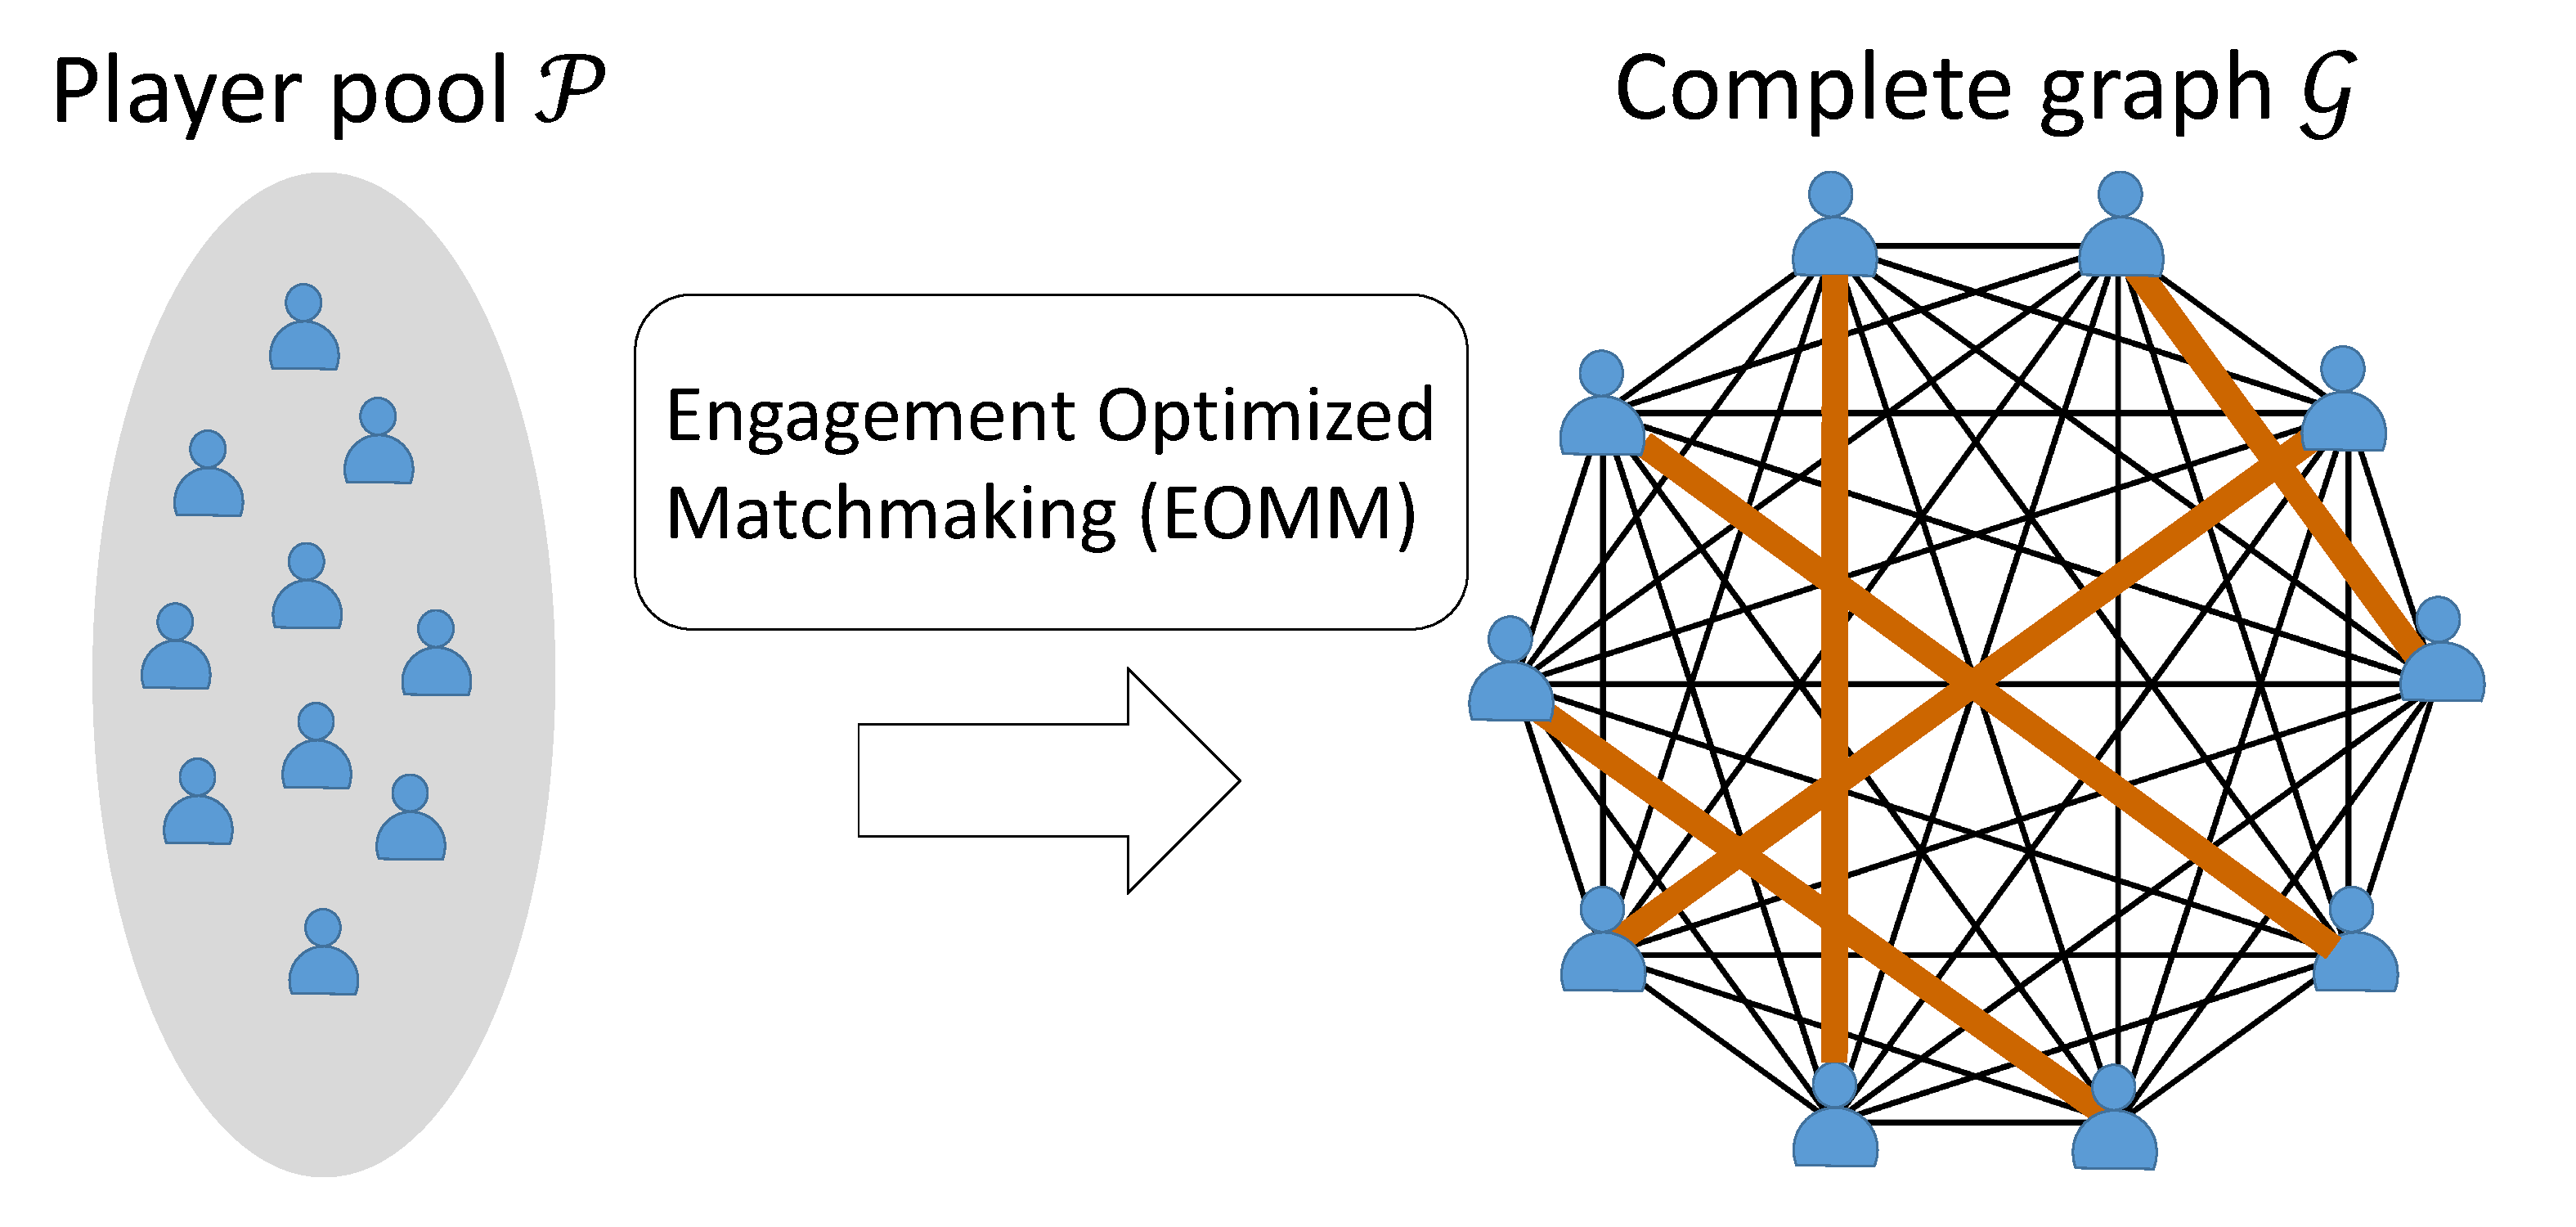
\includegraphics[width=1\textwidth]{Figures/complete_matching.pdf}
\caption{Model matchmaking on a complete graph. Each node represents a player, and every edge is associated with the sum engagement metric of two players if paired. EOMM amounts to finding an optimal pair assignment on $\mathcal{G}$.}
\label{fig:matching}
\end{figure}


\subsection{Predicting Churn Risks}\label{sec:churn}
We learn the function $c_{i,j} = c(\vect{s}_i, \vect{s}_j)$ as a churn prediction problem. In its original form, the churn risk $c_{i,j}$ of player $p_i$ after matchmaking depends on the states from both the player and their opponent. Unfortunately, the well-established churn prediction studies cannot be employed here, because they only use features of players themselves without considering those of opponents. Also, naively feeding both player states as input will double the feature dimension, which makes the prediction unintelligible and harder since much more training data is needed. 

One way to simplify the prediction of $c_{i,j}$ is to base it only on player $p_i$'s own state, $\vect{s}_i$, and the resulting match outcome, $o_{i,j}$, from the view of $p_i$. This works because the opponent's state, $\vect{s}_j$, such as skill, play history and style, does not directly interact with player $p_i$'s churn risk $c_{i,j}$. It, however, influences the upcoming match outcome, which is directly perceivable by player $p_i$ and thus affects $p_i$'s churn. Once the match outcome $o_{i,j}$ is known, $c_{i,j}$ becomes conditionally independent to the opponent's state, $\vect{s}_j$. Formally, this property is represented as:
\begin{equation}\label{eqn:dependency_raw}
\Pr(p_i \text{ churns} | \vect{s}_i, \vect{s}_j, o_{i,j}) = \Pr(p_i \text{ churns} | \vect{s}_i, o_{i,j}),
\end{equation}
which can be written in a concise form:
\begin{equation}\label{eqn:dependency}
c(\vect{s}_i, \vect{s}_j, o_{i,j}) = c(\vect{s}_i, o_{i,j})
\end{equation}

In this chapter, we assume that game outcomes are sampled from a finite set, $\mathcal{O}$, such as \emph{Win}, \emph{Lose} and \emph{Draw}. For example, $o_{i,j}=W$ means that $p_i$ wins over $p_j$, while $o_{j,i}=L$ represents the same outcome from the view of $p_j$. To predict game outcomes, we employ the standard skill models~\cite{elo1978rating,glickman1999parameter} that are widely adopted in the video game industry. These models use both players' skills, which are a proxy of their entire player states, as the input for the prediction. We denote player $p_i$'s skill representation as $\vect{\mu}_i$, which is, for example, Elo score~\cite{elo1978rating} or Glicko mean and RD~\cite{glickman1999parameter}. Note that $\vect{\mu}_i$ is part of player state $\vect{s}_i$.  As a result, we have:
\begin{equation}\label{eqn:skill}
\Pr(o_{i,j}|\vect{s}_i, \vect{s}_j) \approx \Pr(o_{i,j}|\vect{\mu}_i, \vect{\mu}_j),
\end{equation}

Putting them together, we can efficiently predict the churn risks of paired players in Eqn.~\ref{eqn:opt2}:
\begin{align}
&c(\vect{s}_i, \vect{s}_j) + c(\vect{s}_j, \vect{s}_i) \label{eqn:c1} \\
=& \sum\limits_{o_{i,j} \in \mathcal{O}} \Pr(o_{i,j}|\vect{s}_i, \vect{s}_j)\left( c(\vect{s}_i, \vect{s}_j, o_{i,j}) + c(\vect{s}_j, \vect{s}_i, o_{j,i}) \right) \label{eqn:c2} \\
\approx & \sum\limits_{o_{i,j} \in \mathcal{O}} \Pr(o_{i,j}|\vect{\mu}_i, \vect{\mu}_j)\left( c(\vect{s}_i, o_{i,j}) + c(\vect{s}_j, o_{j,i}) \right), \label{eqn:c3}
\end{align}
where the first equality is a marginalization on game outcome, $o_{i,j}$. In the approximate equality, the conditional independence of $c_{i,j}$ on $\vect{s}_j$ given $o_{i,j}$ (Eqn.~\ref{eqn:dependency}) and the game outcome prediction (Eqn.~\ref{eqn:skill}) are used.

Now $c(\vect{s}_i, o_{i,j})$ can be efficiently learned based on any preferred churn prediction model. The input features are the updated player state based on the predicted game outcome of the hypothetical matchmaking, i.e., $\vect{s}_i^{update} \leftarrow \vect{s}_i \text{ and } o_{i,j}$. We can decompose the original player state as $\vect{s}_i = [\vect{o}_i^K, \hat{\vect{s}}_i]$, where $\vect{o}_i^K$ is a vector of the latest $K$ game outcomes (for example, $\vect{o}_i^K=LWLDL$ when $K=5$), and $\hat{\vect{s}}_i$ represent the rest of features in $\vect{s}_i$. If $p_i$ is hypothetically matched with $p_j$, $\vect{s}_i$ will be updated as:
\begin{align}\label{eqn:stateUpdate}
\vect{s}_i^{update} \leftarrow& \vect{s}_i \text{ and } o_{i,j} \\
                    =& [\vect{o}_i^K, \hat{\vect{s}}_i] \text{ and } o_{i,j} \\
                    =& [\vect{o}_i^{K+1}, \hat{\vect{s}}_i^{update}]
\end{align}
We use $\hat{\vect{s}}_i^{update}$ to indicate that non-game-outcome features are also updated after the new match. For example, the total number of games played increments by one. 


%Then, we can adopt any preferred churn prediction model based on $\vect{s}_i^{update}$ in order to compute $c(\vect{s}_i, o_{i,j})$.
\vspace{2mm}

\subsection{Finding the Optimal Pair Assignment}
Given the predicted churn risks of each pair of players, i.e., the weight of every edge in $\mathcal{G}$, EOMM reduces to a minimum weight perfect matching (MWPM) problem. The goal is to find a pair assignment, $\mathcal{M}^*$, on a complete graph, $\mathcal{G}$, which has the minimal sum weights of edges.

For a graph with $N$ node, the brute-force method is to compare all $\binom N{N/2} / 2^{\frac{N}{2}}$ possible pair assignments and find the best one, but the time complexity is too high to be feasible in practical systems. Fortunately, many polynomial time algorithms exist for the MWPM problem. For example, several algorithms can solve the problem in the worst time complexity $O(N^3)$ \cite{gabow1974implementation,lawler2001combinatorial}. If engagement measurements are pure integers, there exists a slightly faster algorithm \cite{gabow1985scaling} with running time $O(N^{2\frac{3}{4}}\log K)$ where $K$ is the largest magnitude of an edge weight. There also exist greedy algorithms, such as \cite{drake2003simple} and \cite{duan2014linear}, with faster running time to find suboptimal solutions. Moreover, MWPM can be solved in parallel as proposed by \cite{osiakwan1990maximum}.

\vspace{3mm}

\section{Theoretical Findings}\label{sec:findings}
Besides generating optimal matchmaking assignments, EOMM provides a framework to conduct theoretical analysis on other matchmaking related problems. We use this framework to compare EOMM with other matchmaking strategies under different hypothetical situations to obtain many insights. Without loss of generality, we focus our discussion on 1-vs-1 games with possible game outcomes sampled from \emph{Win}, \emph{Lose} and \emph{Draw}.

Using the same notation in Section~\ref{sec:optimization}, we investigate a pair of players $p_i, p_j \in \mathcal{P}, i \neq j$. When $c(\vect{s}_i, \vect{s}_j) = c(o_{i,j})$, i.e., a player's churn risk only depends on the game outcome of the upcoming match, regardless of all other states. This simplification for Eqn.~\ref{eqn:stateUpdate}, where $\vect{s}_i^{update}$ only considers $o_{i,j}$ but ignores $\vect{s}_i$, has  interesting implications.
\begin{itemize}
\item If $c(Win)+c(Lose) > 2\cdot c(Draw)$, i.e., the sum churn risk of two matched players in a tied game is lower than that in a non-tied game. Under this circumstance, the equal-skill based matchmaking is \emph{equivalent} to EOMM, as both strive to form matches with \emph{Draw} outcomes as many as possible. This explains the intuition and popularity behind equal-skill matchmaking. But we should be aware of its conditional applicability, while EOMM is instead always optimal.
\item If $c(Win) + c(Lose)< 2\cdot c(Draw)$, equal-skill based matchmaking is actually \emph{worst} among all matchmaking schemes, as its goal to create close matches contrarily minimizes the overall player engagement. Although this situation contradicts with the common intuition that fair matches are good, it is possible for a real game. Therefore, validating the assumptions with real game data is critical before applying an equal-skill based matchmaking algorithm.
\end{itemize}

When $c(\vect{s}_i, \vect{s}_j) = c(\vect{s}_i)$, i.e., a player's churn risk is determined by his state before matchmaking, then it does not matter whom they will play. In this case, EOMM can do no better than a random matchmaking. Random matchmaking, from this perspective, is not trivial. It is a relative safe and stable baseline choice in lack of prior information. While equal-skill based method can perform the worst under certain conditions, random matchmaking will never fall into the worst case.

The analysis above shows that the existing matchmaking methods, such as equal-skill based and random matching, arise within the EOMM framework on different conditions. Practitioners can safely apply EOMM while gathering more information about their game and players.

\section{Case Study}\label{sec:casestudy}
To test the proposed matchmaking framework, we ran simulation which is configured based on the real data from a popular PvP game made by Electronic Arts Inc.\! (EA). In the simulation, we compared different matchmaking methods applied to the same player population. In the end, EOMM retained significantly higher number of players than other matchmaking methods.

\subsection{Data Collection}
We collected 1-vs-1 matches from a popular game made by EA. There are three possible match outcomes, namely \emph{Win}, \emph{Lose} and \emph{Draw}. In total, we collected 36.9 million matches played by 1.68 million unique players in the first half of 2016.

\subsection{Preparation}\label{sec:preprosessing}

\begin{figure}[t]
\centering
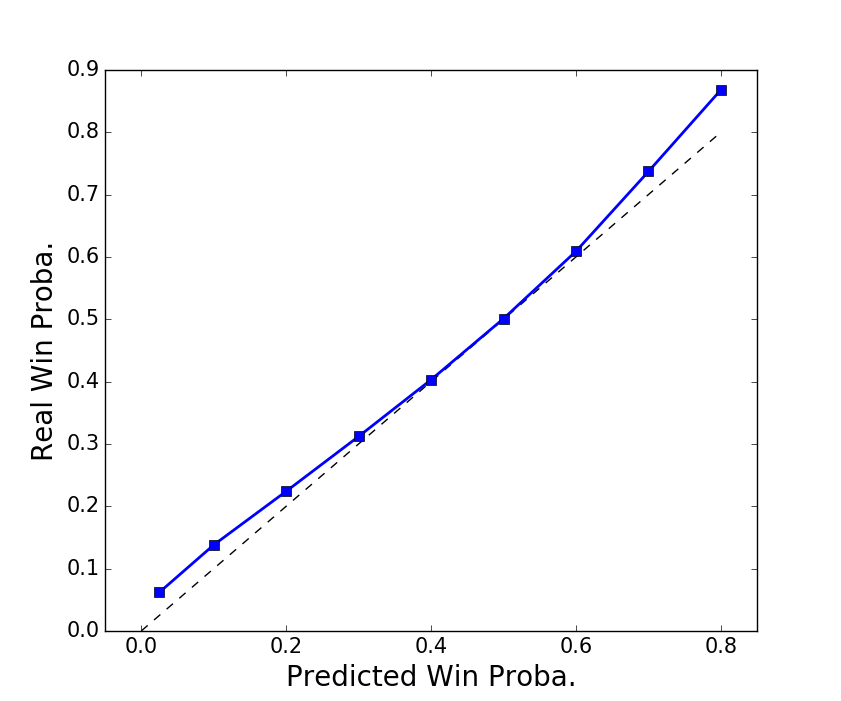
\includegraphics[width=0.8\textwidth]{Figures/prob_calib_glicko_line.png}
\caption{Predicted win probability vs. real win probability. Real win probability is the ratio of matches, with similar predicted winning probabilities, whose outcomes are real ``Wins''.  }
\label{fig:glicko_cali}
\end{figure}


To create a realistic environment for simulation, the following models and functions are needed. We compute them based on real game data.

\textbf{Player Skills} We need to establish a distribution of player skills for the population we simulate on. The distribution is learned from real game data. We sorted the collected real matches temporally and applied Glicko~\cite{glickman1999parameter} to compute each player's final skill. For each player $i$, the skill vector is represented by mean $r_i$ and variance $RD_i$, i.e. $\vect{\mu}_i = (r_i, RD_i)$. In simulation, we assume that the game and player skills are stationary. The population's skill distribution is constant, where each player's skill does not change any more over time.

% We chose to update Glicko ratings of involved players after every match. The estimated player skills were stored in a HashMap-like data structure indexed by player identities.

While Glicko scores can be used to estimate the winning probability of player $i$ over player $j$, $\Pr(i > j | \vect{\mu}_i, \vect{\mu}_j)$, they cannot provide the probability of draws. We defined a set of rules to allow the estimation of win/lose/draw probabilities from Glicko scores:
\begin{align}\label{eqn:draw}
\text{Pr}^*(i=j) = 20\%
\end{align}

\begin{align}
\text{Pr}^*(i>j)  = \frac{80\% \cdot \Pr(i > j | \vect{\mu}_i, \vect{\mu}_j)}{\Pr(i > j | \vect{\mu}_i, \vect{\mu}_j) + \Pr(j > i | \vect{\mu}_j, \vect{\mu}_i) }
\end{align}

\begin{align}
\text{Pr}^*(i<j) = 1 - \text{Pr}^*(i=j) - \text{Pr}^*(i>j)
\end{align}

% All the roofs of the bars are around the diagonal (dashed line), suggesting predicted win ratios by our rules are well calibrated.
Basically, the draw probability (Eqn.~\ref{eqn:draw}) is set to $20\%$ regardless of skill gaps. This is based on our findings that 1) draw outcomes only have $-0.05$ correlation with the difference of skill means in the collected game data; 2) around $20\%$ matches are draws regardless of skill gaps. The win/lose probabilities are normalized such that the probabilities of win, lose and draw sum up to 1. Figure~\ref{fig:glicko_cali} shows that the predicted win probabilities using Glicko scores based on our rules are well aligned with the real match outcomes.

\textbf{Churn Prediction Model} We trained a logistic regression model for predicting whether a player will be an eight-hour churner after a match. The input features describe the upcoming match and the player's 10 most recent matches. A player is labeled as an eight-hour churner if they do not play any 1-vs-1 match within the next eight hours after playing this match. As discussed in Section~\ref{sec:optimization}, the term of ``churn'' is used by convention. It represents ``stopping playing'' within a period of time, which is a metric of disengagement.

\begin{figure}[t]
\centering
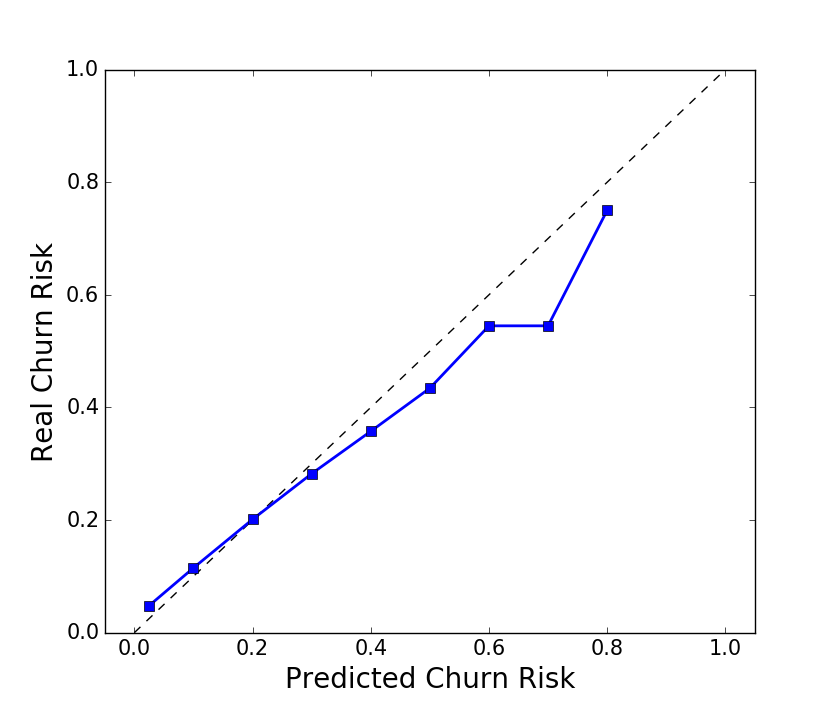
\includegraphics[width=0.8\textwidth]{Figures/prob_calib_lr_line.png}
\caption{Predicted churn risk vs. real churn risk. Real churn risk is the ratio of matches, with similar predicted churn risks, which are indeed the last match before churn. }
\label{fig:lr_cali}
\end{figure}

We use Eqn.~\ref{eqn:c3} to estimate $c(\vect{s}_i, \vect{s}_j) + c(\vect{s}_j, \vect{s}_i)$. The model takes as input the player's state $\vect{s}_i$ before matchmaking along with the upcoming match outcome $o_{i, j}$.

Specifically, the input features consist of:
\begin{itemize}
\item \textit{Each of the player's 10 most recent matches}: win/lose/draw status, time passage since the previous match, time passage to the upcoming match, and goal difference against his opponent
\item \textit{Upcoming match}: one-hot encoding of the upcoming match's outcome win/lose/draw
\item \textit{Other}: the number of 1-vs-1 matches played in the last eight hours, one day, one week and one month.
\end{itemize}

%The size of extracted data points after random sampling is 10 million. The ratio between positive (churned) and negative (not churned) labels is approximately 1:3.
% The range of grid search is from $10^{-3} \sim 10^3$.
% The performance of the best model (in terms of F1 score) is listed in Table 3 (averaged over 5 hold-out sample sets).

We use 5-fold cross validation and grid search to determine the proper $L_2$ regularization strength when training the model. The predicted probabilities are well aligned with the real churn probabilities, in particular when churn risk is less than 0.8, as shown in Figure~\ref{fig:lr_cali}. While the performance of the predictive model still has room to improve, the flexibility of EOMM allows one to easily refine or replace the model if better ones are found.

%One can easily notice that the recall of the best model is very low. This is due to the skewness of  labels of the dataset and the insufficient power of selected features to capture  churn patterns. To train a churn model performing more accurate classification, one can incorporate weights for data points \cite{lee2003learning} \footnote{if we adjust weights of data points inversely proportional to class frequencies in the input data, we can obtain a logistic regression model with 60.96\% accuracy, 66.66\% AUC, 63.65\% recall, 34.35\% precision and 0.4462 F1-score. (All metrics are averaged over 5 hold-out sample sets.)}, conduct more sophisticated feature engineering and test with more advanced models. However, the most important property of an engagement predictive model desired by EOMM should be that its predicting probabilities are well calibrated such that $G(\vect{s}_i, \vect{s}_j)$ is unbiased. We should think the logistic regression model as a churn risk estimator, rather than an accurate binary classifier. Since the logistic regression model directly optimizes for log-likelihood, its prediction probabilities are well aligned with real data, as shown in Figure~\ref{fig:lr_cali}. Therefore, we think the trained model is desirable in this case study primarily as an illustration of the applicability of EOMM.



%
%\begin{table}[]
%\centering
%\ra{1.1}
%\caption{Performance Evaluation on Churn Prediction Model}
%\begin{tabular}{ccccc}
%\hline
%Accuracy & AUC & Recall & Precision & F1-Score\\ \hline
%75.23\% & 64.21\% & 3.48\%  & 48.18\% & 0.0650 \\ \hline
%\end{tabular}
%\end{table}
% AUC is close to other papers?


\textbf{Player States} In simulation, each player's state is sampled from a collection of states, which are established based on real players' states in the collected data. We first randomly sample a subset of matches. Both players' states in those matches are gathered to create this collection. A player state contains the needed features for churn prediction, as well as the player's skill score.

% In total, the size of the player state sample pool is 10 million.
%We avoided player state samples or training data for the engagement prediction model that less than 15 recent matches are available for a player to be filled in. One should acknowledge that dealing with casual players is hard in practice and it is out of our scope.

%\newpage
\subsection{Simulation Procedure}
In the simulation, we compared EOMM with three matchmaking mechanisms: \textit{random matchmaking} (\textit{RandomMM}), which randomly pairs available players in the waiting pool, \textit{skill-based matchmaking} (\textit{SkillMM}), which pairs every two consecutive players after sorting them by skills, and \textit{worst matchmaking} (\textit{WorstMM}), which does the opposite of EOMM by minimizing the objective function of EOMM. SkillMM always seeks ``fair games''. We added WorstMM as a validation.

All methods are applied on the same population (waiting pool), where the same player skill distribution, churn model and player state distribution as described in Section~\ref{sec:preprosessing} are used. EOMM follows Eqn.~\ref{eqn:c3} to estimate churn risk $c(\vect{s}_i, \vect{s}_j) + c(\vect{s}_j, \vect{s}_i)$. We used the perfect matching algorithm \cite{gabow1974implementation,lawler2001combinatorial} implemented by an open-source library \cite{onlineperfectmatching}.



For each matchmaking method $\mathcal{M}$, the procedure within each round of simulation is as follows:
\begin{enumerate}
\item Create a waiting pool of $P$ players, whose player states are sampled from the player state collection.
\item Use $\mathcal{M}$ to determine the pair assignment (matchmaking).
\item Simulate match outcomes according to the win/lose/draw probability predicted by the skill model
\item For each player, simulate if he will churn according to the predicted churn probability by churn model.
\item Record the number of retained players.
\end{enumerate}

In experiments, we tested $P=100, 200, 300, 400$ and $500$. For each setting of $P$, we repeated the simulation by 10,000 rounds of matchmaking. We compare different matchmaking methods by the average number of their retained players per round, i.e., the players who continue playing in the next eight hours. In order to test statistical significance, we conducted Welch's $t$-test between every pair of the matchmaking algorithms.

%\begin{table*}[]
%\centering
%\ra{1.1}
%\caption{P-Values of Pairwise Welch's T-Tests}
%\begin{tabular}{lccccc}
%\hline
%\multicolumn{1}{c}{Method}                  & \multicolumn{5}{c}{p-value}    \\
%& \multicolumn{1}{c}{N=100} & \multicolumn{1}{c}{N=200} & \multicolumn{1}{c}{N=300} & \multicolumn{1}{c}{N=400} & \multicolumn{1}{c}{N=500} \\ \hline
%EOMM vs. WorstMM        & 1.83e-08**  & 2.24e-20**  & 6.25e-133**  & 3.45e-77**  & 2.36e-84** \\ \hline
%EOMM vs. SkillMM        & 1.43e-18**  & 2.84e-03**  & 1.95e-33**   & 3.55e-40**  & 2.50e-37** \\ \hline
%EOMM vs. RandomMM       & 2.16e-01  & 3.82e-03**  & 2.86e-33**   & 2.28e-53**  & 3.77e-23** \\ \hline
%SkillMM vs. WorstMM     & 6.73e-48**  & 5.62e-10**  & 1.19e-33**   & 2.55e-08**  & 1.08e-11** \\ \hline
%SkillMM vs. RandomMM    & 8.89e-24**  & 9.23e-01**  & 7.52e-01   & 1.71e-02*  & 5.98e-03** \\ \hline
%RandomMM vs. WorstMM    & 1.14e-05**  & 2.77e-10**  & 6.51e-37**   & 1.88e-03**  & 3.03e-21** \\ \hline
%\end{tabular}
%\end{table*}






\subsection{Results and Discussion}

The results are shown in Table~\ref{tab:result}. All pairwise differences of retained players are statistically significant ($p$-value $< 0.01$) except EOMM vs.\! RandomMM (when $P=100$) and SkillMM vs.\! RandomMM (when $P=400$). In all other scenarios, EOMM outperforms the other three matchmaking methods. The results prove the applicability of EOMM to act as an engagement optimizer. When $P=100$, EOMM does not retain a significantly higher number of players than RandomMM, and even retains fewer players than SkillMM. It is possibly because that when $P$ is small, the randomness has higher impact, and also, the room for arranging opponents is smaller. More rounds of simulations might be needed to show significance in this case.

The improvement of EOMM over SkillMM, the most common matchmaking method, in terms of the average number of retained players are $0.3\%$, $0.9\%$, $1.1\%$, and $0.6\%$ when $P=200, 300, 400$ and $500$ respectively. On average EOMM retains $0.7\%$ more player compared with SkillMM after one round of matchmaking. Notably the benefit of retention will accumulate over time in a constant population. For players who play 20 rounds of matchmaking games within eight hours, there will be $15\%$ more players retained ($1.007^{20}$ $ \approx 1.15$) by EOMM over those by SkillMM. The more rounds of matchmaking are conducted, the more significant is the accumulative advantage of EOMM in engagement.

We did not find a consistent climb in retention boost as $P$ increased. This may suggest that when the player pool reaches certain size, the choices of opponents are enough to rescue those players on the edge of churn. Beyond this size, a larger player pool may not bring in significantly extra benefits in engagement maximization.

As a validation, WorstMM consistently retains the fewest players in the pools of all sizes. This result verifies the optimum of EOMM from the opposite side. It is also interesting to note that SkillMM does not consistently outperform RandomMM, which is aligned with our discussion in the theoretical findings in Section~\ref{sec:findings}, that is, balanced matches are not always optimal for engagement.


\begin{table}[t]
\centering
\ra{1.1}
\caption{Average number of retained players per round of matchmaking simulation. 10,000 rounds of matchmaking were simulated.}
\label{tab:result}
\begin{tabular}{lccccc}
\hline
\emph{Method} & \multicolumn{1}{c}{P=100} & \multicolumn{1}{c}{P=200} & \multicolumn{1}{c}{P=300} & \multicolumn{1}{c}{P=400} & \multicolumn{1}{c}{P=500} \\ \hline
WorstMM  & 51.50   & 103.39   & 154.57    & 206.65  &  258.21  \\ \hline
SkillMM  & 52.52   & 103.96   & 156.05    & 207.43  &  259.24  \\ \hline
RandomMM & 51.81   & 103.97   & 156.09    & 207.09  &  259.65  \\ \hline
EOMM     & 51.90   & 104.24   & 157.50    & 209.37  &  261.19  \\ \hline
\end{tabular}
\end{table}



\section{Summary}
This chapter attempts to answer \hyperref[rq2]{\textbf{R.S.Q.~2}} by presenting a novel framework, Engagement Optimized Matchmaking (EOMM), to achieve optimized engagement for a population of online players through recommendation of opponents. It formulates matchmaking as a problem of maximizing the player engagement, and solves the optimization efficiently. EOMM employs three components, a skill model, an engagement predictive model and a minimum weight perfect matching algorithm, each of which can be tailored flexibly for specific applications. We ran simulations whose configurations were based on real data from an online PvP game. The results show that EOMM significantly outperforms all other methods in the number of retained players. EOMM also provides a theoretical framework to analyze various matchmaking algorithms.

EOMM provides a measurable and flexible matchmaking framework. It has well-defined quantitative objectives that can be monitored, evaluated and improved. Within the EOMM framework, the core building components, skill model, churn model and graph pairing model, are uncoupled so that they can be tuned and replaced independently. Moreover, we can even change the objective function to other data-driven metrics of player engagement, such as play time, retention, or spending. EOMM allows one to easily plug in different types of predictive models to achieve the optimization.

% So far we have discussed EOMM in 1-vs-1 game scenarios. This framework also applies to PvP games that involve teams of players, where every component needs to be extended with additional care. The skill model can be simply applied to a team by adding up skills for all team members~\cite{herbrich:trueskill}. For churn prediction, we can use the same idea that one player's churn risk is conditionally independent with other players' states given that their influence on the player's own state, such as the game outcome, is known. Last, the minimum weight perfect matching algorithms for pairs are no longer applicable. Instead of a pair assignment, we seek a \emph{grouping assignment} on a complete graph. A related area to investigate is perfect matching in hypergraphs~\cite{berge1984hypergraphs}, where an edge can connect more than two vertices. Furthermore, EOMM is not even limited to games. In broad applications, such as friend connection in a social network and 1-on-1 tutoring in online education, EOMM's formulation and optimization techniques still apply.

% In the future, we expect EOMM equipped with more advanced models, such as skill model and churn model, can have higher optimal bound. We will explore EOMM performance in more realistic situations, where practical restrictions are applied, such as network connectivity, regions and friend/black lists. More restrictions would result in fewer edges in the constructed graph of EOMM. Last, we will explore EOMM in multi-player games with more than two players involved and efficient algorithms analogous to perfect matching algorithms within hypergraphs.